\documentclass[12pt]{article}

\input{C:/Users/ilden/Documents/School/TeX памятка/header.tex}

\begin{document}
	\tableofcontents
	\setcounter{tocdepth}{3}
	\newpage
	\section{Правила дорожного движения и ДТП.}
	\begin{definition}
		ДТП~--- это событие, возникшее в процессе движение по дороге транспортного средства и с его участием, при котором погибли или пострадали люди, повреждены транспортные средства, сооружения, грузы или причинен иной материальный ущерб.
	\end{definition}
	\subsection{Участники дорожного движения.}
	\begin{itemize}
		\item Пешеход.
		\item Водитель.
	\end{itemize}
	\subsection{Фактор риска возникновения ДТП.}
	\begin{itemize}
		\item Нарушение ПДД.
		\begin{itemize}
			\item Превышение скорости.
			\item Проезд на запрещающий свет светофора.
			\item Не соблюдение дистанции.
		\end{itemize}
		\item Погодные условия и время суток.
		\begin{itemize}
			\item Снегопад.
			\item Лед.
			\item Дождь.
			\item Темное время суток.
			\item Яркий солнечный свет.
		\end{itemize}
		\item Состояние дорожного покрытия.
		\item Техническая неисправность транспортного средства.
		\begin{itemize}
			\item Отказ тормозной системы.
			\item Износ шин.
			\item Неисправность рулевого управления.
			\item Проблемы с фарами.
		\end{itemize}
	\end{itemize}
	\subsection{Знаки дорожного движения.}
	\subsubsection{Виды знаков дорожного движения.}
	\begin{itemize}
		\item Предупреждающие знаки. Чаще всего имеют треугольную форму с белым фоном и красной рамкой. Исключения~--- знаки, которые показывают о железнодорожном переезде или направлении поворота.
		\begin{figure}[H]
			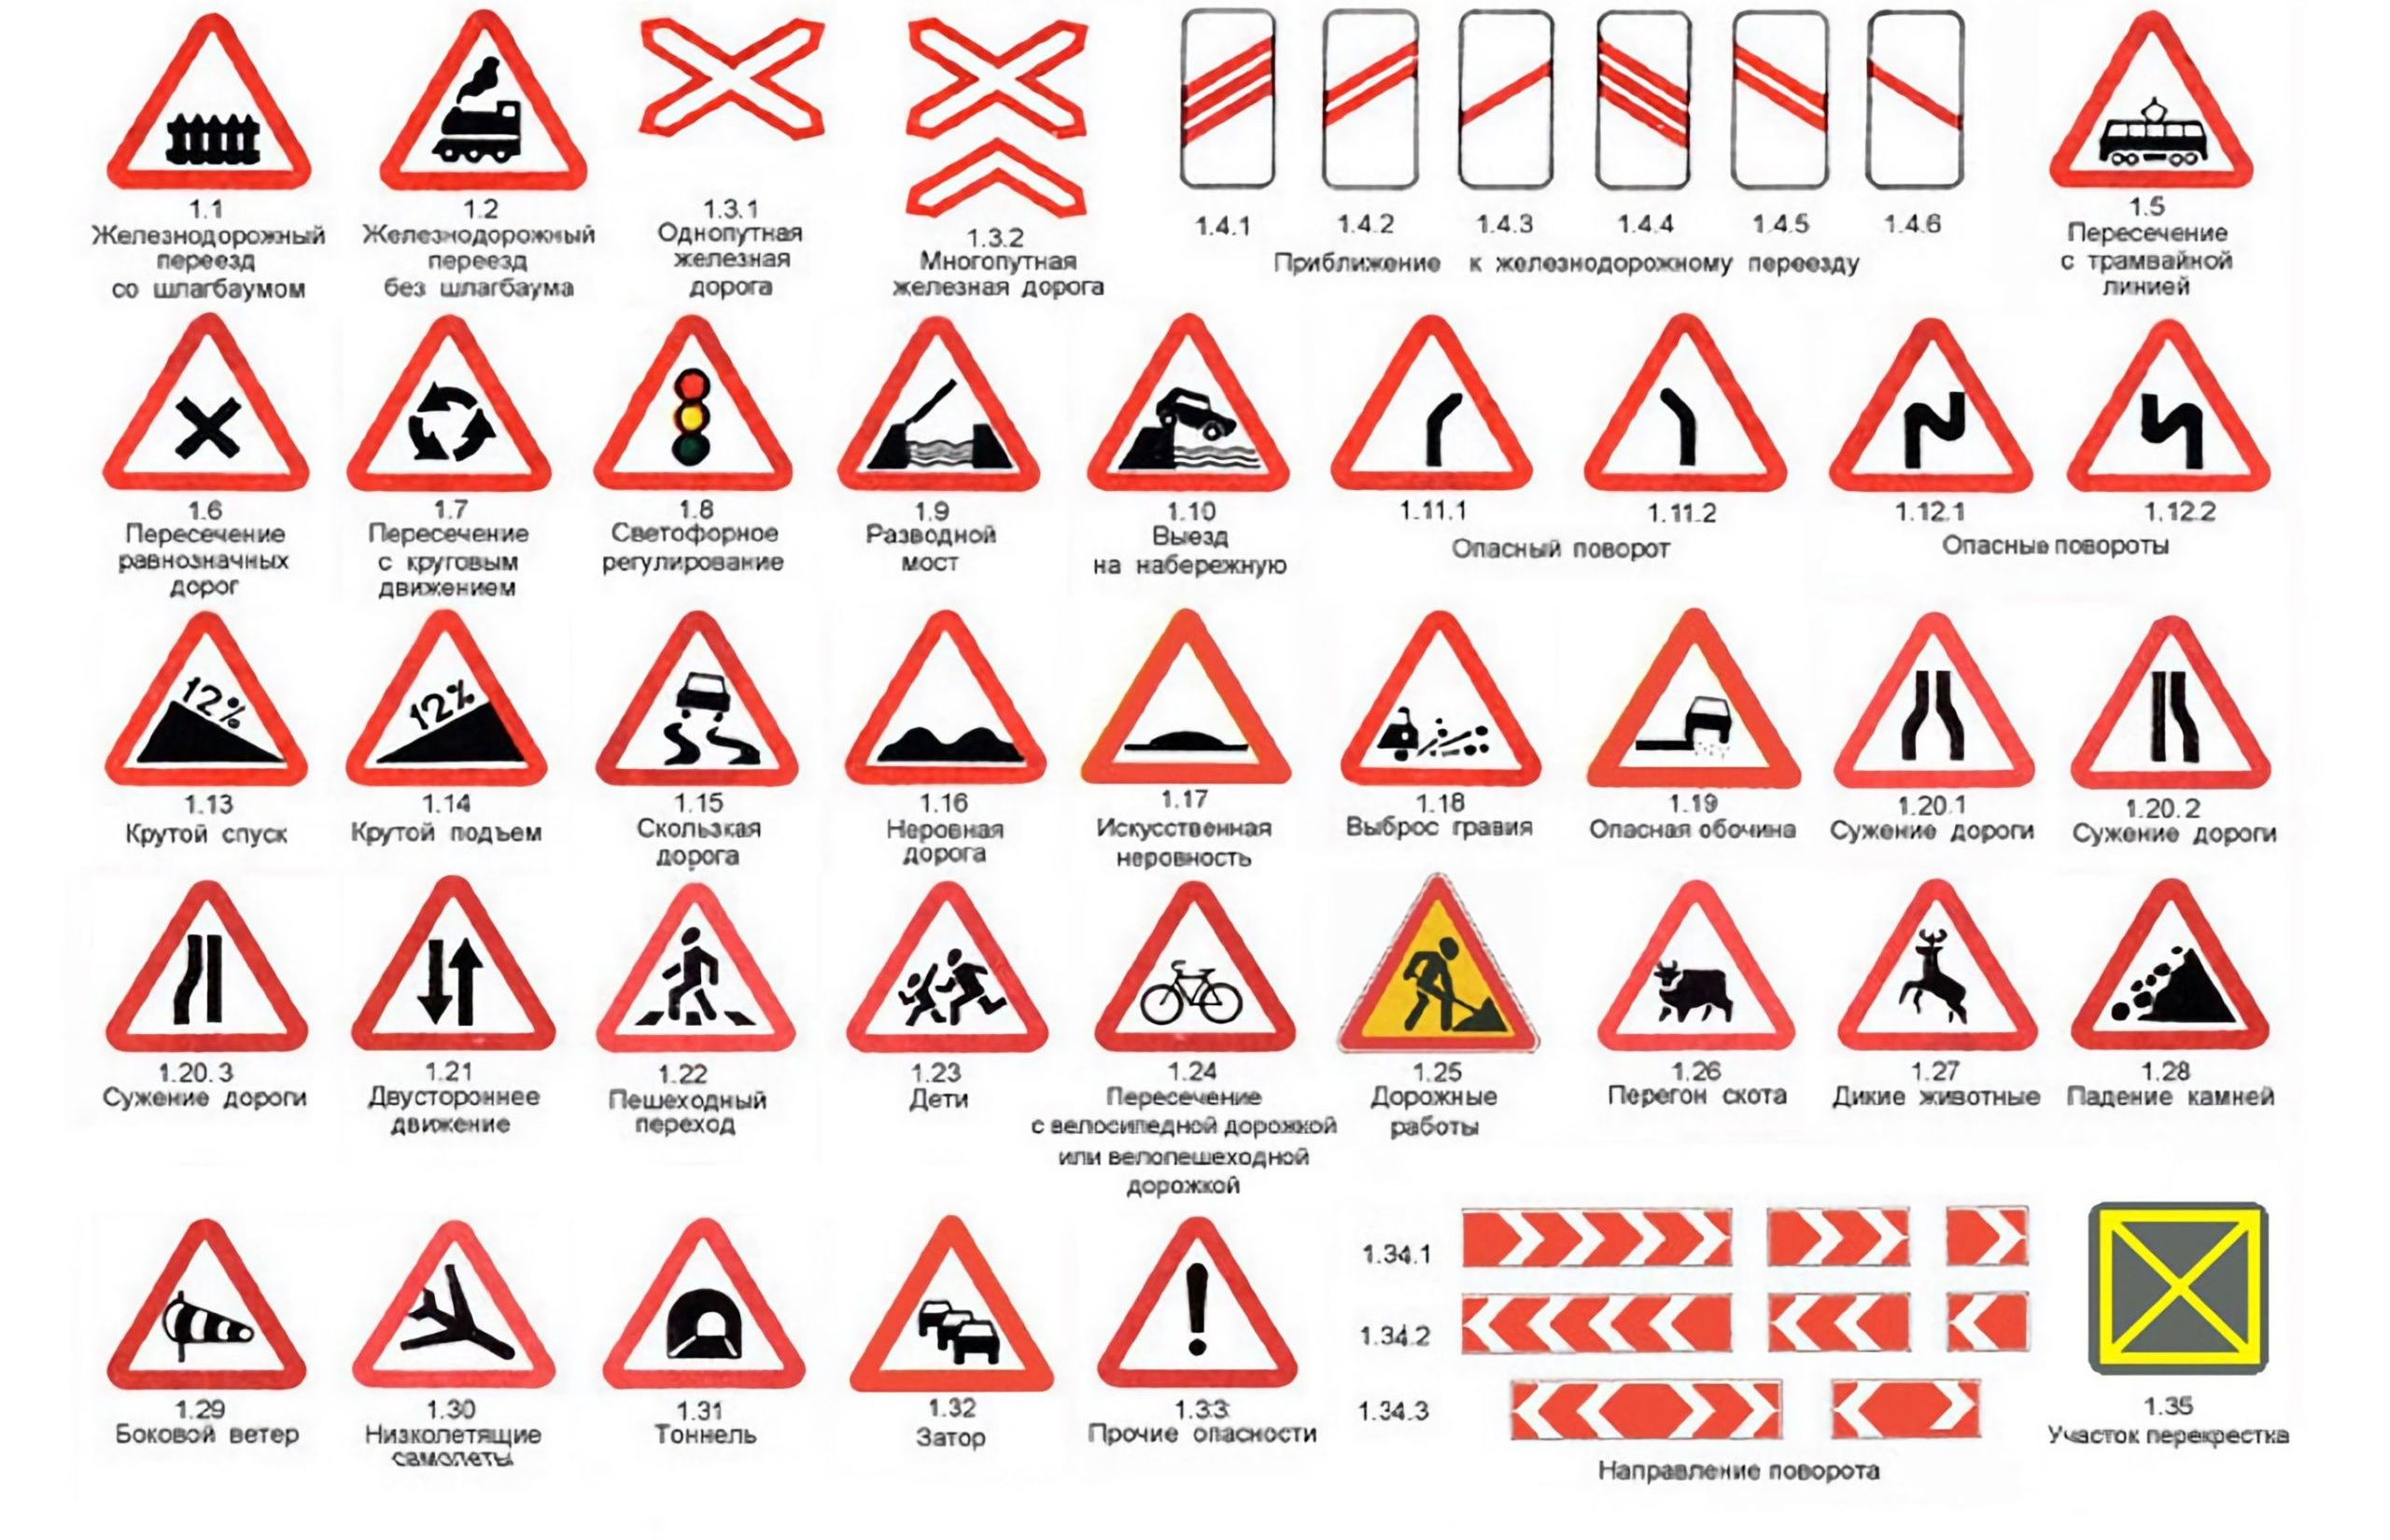
\includegraphics[height=0.6\textwidth]{extra-materials/Предупреждающие-знаки-ПДД}
			\caption{Предупреждающие знаки ПДД.}
		\end{figure}
		\item Запрещающие знаки. Имеют круглую форму.
		\begin{figure}[H]
			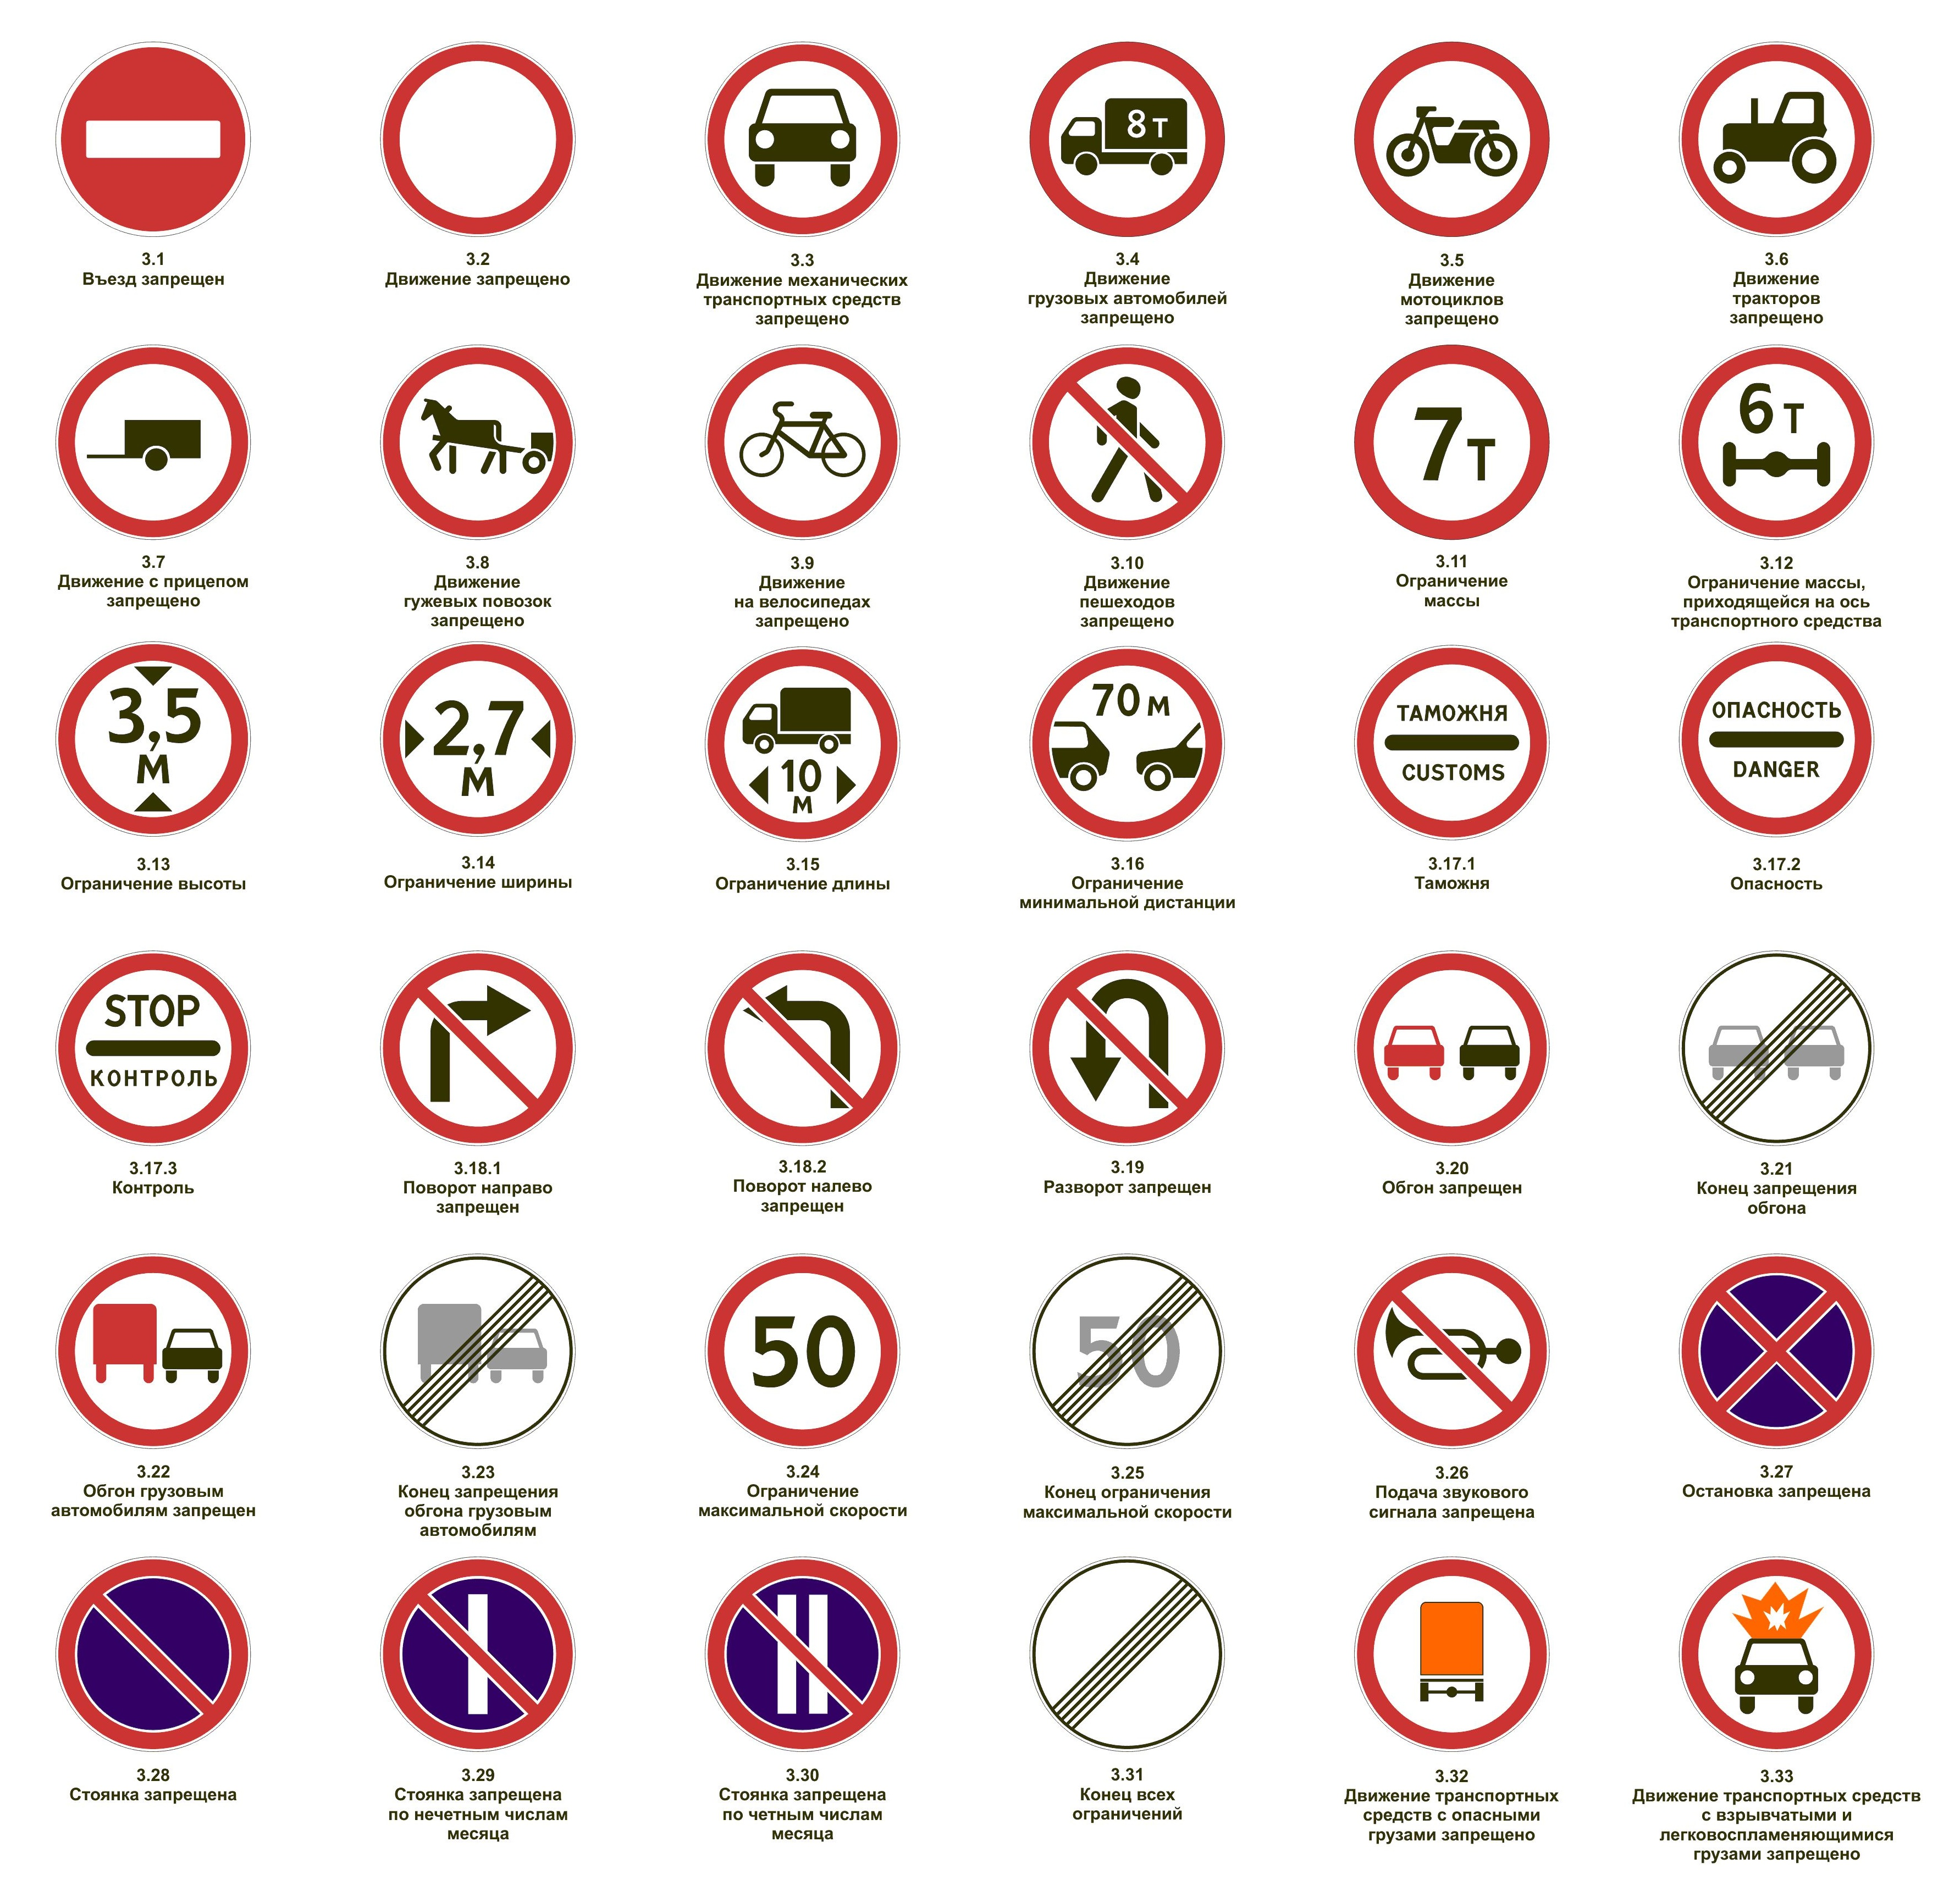
\includegraphics[height=0.55\textwidth]{extra-materials/Запрещающие-знаки-ПДД}
			\caption{Запрещающие знаки ПДД.}
		\end{figure}
	\end{itemize}
\end{document}
